% \documentclass[CEJM,DVI]{cej} % use DVI command to enable LaTeX driver
\documentclass[CEJM,PDF]{cej} % use PDF command to enable PDFLaTeX driver
\usepackage{layout}
\usepackage{caption}
\usepackage{subfigure}
\title{Objects Recognization Based on On-line Machine Learning}

\articletype{CIS519 Introduction to Machine Learning Project Proposal} % Research Article, Review Article, Communication, Erratum


\author{Shangyi Cheng\inst{}\email{shangyi@seas.upenn.edu}, Yao Chu\inst{}\email{chuyao@seas.upenn.edu}, Chenyang Zhao\inst{}\email{chzhao@seas.upenn.edu}}
\institute{University of Pennsylvania}

\renewcommand{\baselinestretch}{0.8}

\begin{document}

\maketitle
\vspace*{-20pt}
\section{Introduction}
\vspace*{-10pt}
This proposal presents an idea of recognizing feature objects. For a certain class of objects which we decided to use different balls (e.g., soccerball), similar models are learned off-line. After the test accuracy and off-line training dataset number reach a certain level, the objects models can be incrementally learned on-line via previous object models. The goal in on-line learning part is generate a reasonable initial prediction which provides a significant computation cost reduction of new instance input based on the previous learned models. Meanwhile, the algorithm should be optimize global models based on the on-line learning results. The most difficult part for this project will be how to handle the relations between existed models and incrementally inputed instances. 
\vspace*{-20pt}
\section{Analysis of Available Data}
\vspace*{-10pt}
In the dataset of Caltech 256(Griffin, G. Holub, AD. Perona, P.), there are the data of images of four sphere objects (actually four kinds of ball in sports). 98 images of golf, 174 of soccer-ball, 104 of bowling-ball and 98 of tennis-ball. Among images of the same kind(take soccer-ball as example), some of the images have a whole soccer in the middle and filling the image, while in other images(such as a photo of a soccer game), soccer may occupy a small portion in the corner, showing in part or in group. As shown in Figure 1, we decide to use the former kind of data as the training set and the latter as the test set. So our objective is to find the sphere target on the image first, and then classify it to tell which kind of ball it belongs to.

\begin{figure}[htb]
\begin{minipage}[htb]{0.5\linewidth}
\centering
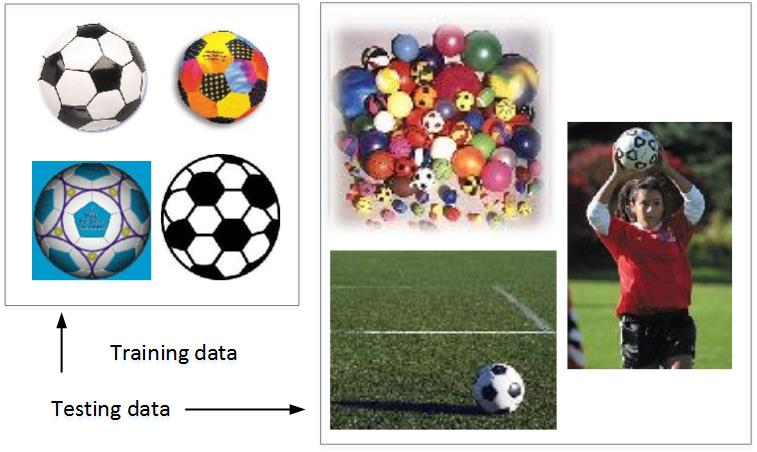
\includegraphics[width=3in]{Analysis_of_Available_Data}
\caption{Analysis of Available Data}
\label{fig:side:a}
\end{minipage}%
\begin{minipage}[htb]{0.5\linewidth}
\centering
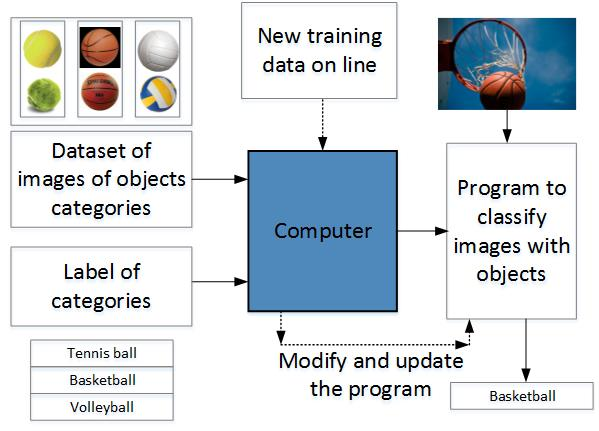
\includegraphics[width=3in]{Expected_Result}
\caption{Expected Result}
\label{fig:side:b}
\end{minipage}
\end{figure}
\vspace*{-45pt}

\section{Machine Learning Methods}
\vspace*{-10pt}
Our goal is decide if a new image contains an instance of our object class or not. According to the previous work by [1], the probability of containing the object can be presented by the features location $\mathbf{X}$, the scales $\mathbf{S}$ and its appearances $\mathbf{A}$, 
\begin{equation}
p(Object) = f(\mathbf{X},\mathbf{S},\mathbf{A},\theta)
\end{equation}
where $\theta$ is the learned parameter of the model. However, when adding a new object class to the learning system, the method needs to start from the initial value $\theta_0$ and iteratively converges to the optimal parameter $\theta$, and the new training data can not contribute to the previous trained data. \\
As described in [2], ELLA maintains a library of k latent model components $\mathbf{L}\in\mathbf{R}^{d\times k}$ shared between tasks. And each task parameter vector $\theta^{(t)}$ could be represented as a linera combination of the columns of $\mathbf{L}$. As new object class $t$ is introduced into the learning system, the matrix of base vectors $\mathbf{L}$ are modified and a new weight vector for this class $\mathbf{s}_t$ is learned by single-task learning algorithm. 
\vspace*{-10pt}

\section{Expected Results}
\vspace*{-10pt}
As shown in Figure 2, with the dataset of several categories of objects(such as various kinds of balls including basketball, baseball, volleyball......), each of which contains 40 - 100 images of the same class, apply the machine learning method described above and it will be able to classify a sphere object contained in a given image. In addition, if we add some new images to the training dataset(either belong to a existing category or a new one), the computer can learn these added data, modify and update the program.

\begin{thebibliography}{9}
\bibitem{p1} Fergus R., Perona P., Zisserman A., Object Class Recognition by Unsupervised Scale-Invariant Learning. Proc. of IEEE Conf on Computer Vision and Pattern Recognition, 2003
\bibitem{ella} Ruvolo, P., and Eaton, E., ELLA: An efficient lifelong learning algorithm. In Proceedings of the 30th International Conference on Machine Learning,2003,  507–515.
\end{thebibliography}

\end{document}